% Options for packages loaded elsewhere
\PassOptionsToPackage{unicode}{hyperref}
\PassOptionsToPackage{hyphens}{url}
%
\documentclass[
  ,
]{article}
\title{Digital media supporting literacy learning in children with
communicative and cognitive disabilities}
\author{true \and true \and true}
\date{28 November, 2022}

\usepackage{amsmath,amssymb}
\usepackage{lmodern}
\usepackage{iftex}
\ifPDFTeX
  \usepackage[T1]{fontenc}
  \usepackage[utf8]{inputenc}
  \usepackage{textcomp} % provide euro and other symbols
\else % if luatex or xetex
  \usepackage{unicode-math}
  \defaultfontfeatures{Scale=MatchLowercase}
  \defaultfontfeatures[\rmfamily]{Ligatures=TeX,Scale=1}
\fi
% Use upquote if available, for straight quotes in verbatim environments
\IfFileExists{upquote.sty}{\usepackage{upquote}}{}
\IfFileExists{microtype.sty}{% use microtype if available
  \usepackage[]{microtype}
  \UseMicrotypeSet[protrusion]{basicmath} % disable protrusion for tt fonts
}{}
\makeatletter
\@ifundefined{KOMAClassName}{% if non-KOMA class
  \IfFileExists{parskip.sty}{%
    \usepackage{parskip}
  }{% else
    \setlength{\parindent}{0pt}
    \setlength{\parskip}{6pt plus 2pt minus 1pt}}
}{% if KOMA class
  \KOMAoptions{parskip=half}}
\makeatother
\usepackage{xcolor}
\IfFileExists{xurl.sty}{\usepackage{xurl}}{} % add URL line breaks if available
\IfFileExists{bookmark.sty}{\usepackage{bookmark}}{\usepackage{hyperref}}
\hypersetup{
  pdftitle={Digital media supporting literacy learning in children with communicative and cognitive disabilities},
  pdflang={english},
  pdfkeywords={Intellectual disability, litteracy learning, phonological
awareness, phonic-based reading strategy, comprehension-based reading,
intervention.},
  hidelinks,
  pdfcreator={LaTeX via pandoc}}
\urlstyle{same} % disable monospaced font for URLs
\usepackage[margin=1in]{geometry}
\usepackage{graphicx}
\makeatletter
\def\maxwidth{\ifdim\Gin@nat@width>\linewidth\linewidth\else\Gin@nat@width\fi}
\def\maxheight{\ifdim\Gin@nat@height>\textheight\textheight\else\Gin@nat@height\fi}
\makeatother
% Scale images if necessary, so that they will not overflow the page
% margins by default, and it is still possible to overwrite the defaults
% using explicit options in \includegraphics[width, height, ...]{}
\setkeys{Gin}{width=\maxwidth,height=\maxheight,keepaspectratio}
% Set default figure placement to htbp
\makeatletter
\def\fps@figure{htbp}
\makeatother
\setlength{\emergencystretch}{3em} % prevent overfull lines
\providecommand{\tightlist}{%
  \setlength{\itemsep}{0pt}\setlength{\parskip}{0pt}}
\setcounter{secnumdepth}{-\maxdimen} % remove section numbering
\newlength{\cslhangindent}
\setlength{\cslhangindent}{1.5em}
\newlength{\csllabelwidth}
\setlength{\csllabelwidth}{3em}
\newlength{\cslentryspacingunit} % times entry-spacing
\setlength{\cslentryspacingunit}{\parskip}
\newenvironment{CSLReferences}[2] % #1 hanging-ident, #2 entry spacing
 {% don't indent paragraphs
  \setlength{\parindent}{0pt}
  % turn on hanging indent if param 1 is 1
  \ifodd #1
  \let\oldpar\par
  \def\par{\hangindent=\cslhangindent\oldpar}
  \fi
  % set entry spacing
  \setlength{\parskip}{#2\cslentryspacingunit}
 }%
 {}
\usepackage{calc}
\newcommand{\CSLBlock}[1]{#1\hfill\break}
\newcommand{\CSLLeftMargin}[1]{\parbox[t]{\csllabelwidth}{#1}}
\newcommand{\CSLRightInline}[1]{\parbox[t]{\linewidth - \csllabelwidth}{#1}\break}
\newcommand{\CSLIndent}[1]{\hspace{\cslhangindent}#1}
\usepackage{setspace}
\AtBeginEnvironment{tabular}{\singlespacing}
\AtBeginEnvironment{lltable}{\singlespacing}
\AtBeginEnvironment{tablenotes}{\doublespacing}
\captionsetup[table]{font={stretch=1.5}}
\captionsetup[figure]{font={stretch=1.5}}
\ifXeTeX
  % Load polyglossia as late as possible: uses bidi with RTL langages (e.g. Hebrew, Arabic)
  \usepackage{polyglossia}
  \setmainlanguage[]{}
\else
  \usepackage[main=]{babel}
% get rid of language-specific shorthands (see #6817):
\let\LanguageShortHands\languageshorthands
\def\languageshorthands#1{}
\fi
\ifLuaTeX
  \usepackage{selnolig}  % disable illegal ligatures
\fi

\begin{document}
\maketitle
\begin{abstract}
(ref:abstract)
\end{abstract}

(ref:abstract) \textbf{Background}:
BLALBLALALBLABLABLABLALBALBLABLABLALB \textbf{Method}: One hundred and
thirty-three adolescents with ID were recruited. The participants were
instructed to train in school for a total of 12 hours. \textbf{Results}:
Blablablablalbalba \textbf{Conclusions}: blablalbalbalbal.

\hypertarget{introduction}{%
\section{Introduction}\label{introduction}}

to be added\ldots{}

\hypertarget{hypotheses}{%
\subsection{Hypotheses}\label{hypotheses}}

1: Training phonic-based or comprehension-based reading strategies
improves phonological awareness. 2: Training phonic-based or
comprehension-based reading strategies improves reading ability. 3: The
combined training is more effective than either intervention on its own.

The hypotheses will be tested on these outcome variables: phonological
awareness (1, 3), word recognition (2, 3), and reading comprehension (2,
3).

\hypertarget{methods}{%
\section{Methods}\label{methods}}

Data presented in this paper is collected in a larger project. Parts of
the data has been used for this paper, for the purpose of this paper we
have excluded for speech sound production which have been published in
Samuelsson et al., (under revision). For a full description of collected
data see (Palmqvist, Samuelsson, et al., 2020).

\hypertarget{participants}{%
\subsection{Participants}\label{participants}}

Inclusion criteria was to attend to a Swedish special needs school, to
benefit from AAC, and to be a beginner at reading. To attend the Swedish
special needs curriculum, the student has received an ID diagnosis after
an assessment led by a licensed psychologist. The teachers were
instructed to identify students that would benefit from AAC and could
not read more than approx. 20 words. No exclusion criteria were set for
age or aetiology of the ID.

The participants were requited via email to teachers at special needs
schools in Sweden. To reduce the risk of having unbalanced groups, the
teachers were asked, together with their notification of interest,
specify how many students in their class that fulfilled the inclusion
criteria and what level of ID the students had. Thereafter, the plan was
for a researcher to allocate the participants on school level to the
different intervention groups. However, only 60 participants were
requited, and data collection had to start due to time constraints.
Thus, the participants could only be assigned to two groups, namely the
comparison and the ALL group. The remainder 77 the participants were
recruited after the data collection of the comparison and ALL group had
started. The participants to the Animega-is and Combination group was
recruited and allocated in the same way as described above. This
resulted in the groups not being equated on level of ID, see the result
section. Caregivers signed an informed consent regarding the
confidentiality of data and group-level analysis. The participating
children gave oral consent at the beginning of the first test session.
The study follows the Ethical principles for medical research involving
human subjects from the WMA Declaration of Helsinki (World Medical
Association 2013). The study was reviewed and approved by the Ethical
Review Board, Sweden (2020-06215).

\hypertarget{design}{%
\subsection{Design}\label{design}}

The study is a longitudinal between-group study, with four time points
(before, during, after the intervention and a follow-up). Three
intervention groups: one applying a phonic-based reading strategy (using
ALL), one applying a comprehension-based strategy (using Animega-is),
and the third applying both strategies (using ALL and Animega-is), and a
comparison group who received regular teaching, not focusing one
specific reading instruction strategy. Due to practical reasons,
students were allocated to intervention groups on school-level, i.e.,
all participants at one school received the same intervention.

\hypertarget{procedure}{%
\subsection{Procedure}\label{procedure}}

Testing took place in a silent environment at the participants' school.
The students were offered to have a teacher or an assistant present
during the assessment. The students' reading ability were assessed at
four times, before (t1), during (t2; approx. at half-time), and after
the intervention (t3) as well as at a 12-week follow-up (t4). For most
of the test situations, t1 and t3 were administered by researchers, t2
and t4 were administered by a special need teacher or a school-based
speech and language pathologist. Data was collected during the
Covid19-pandemic, January 2020 to June 2021, thus, the test
administrators were interchanged as schools introduced restrictions for
visitors. Test administrators practiced the test procedure before data
collection began. Test order was fixed over sessions and students. The
test session lasted \textasciitilde45-75 minutes, including short
breaks. During breaks, students were offered a small snack, water, or to
move around in the room for a few minutes.\\
The literacy training took place in the participants' school. The
teachers were instructed to allow the students to train for 300 minutes
(20 sessions for 15 min, five days a week for four weeks). The teachers
were asked to not assist in solving the tasks for the children. The
teacher was asked to administer the training as they saw fit for each
student, meaning that they were able to split the training sessions into
smaller sessions or train individually, or in group.

\hypertarget{behavioral-measures}{%
\subsection{Behavioral measures}\label{behavioral-measures}}

The participants were assessed on non-verbal intelligence, phonological
awareness, word recognition, and reading comprehension (in that order).
All tests started with two practice items. All tests were adapted so
that the student was able to give a non-verbal response option if
preferred. All instructions were presented verbally in combination with
complementary manual signs and pictures. A test was terminated if the
student gave three consecutive incorrect responses, except for Raven's
where the test was terminated after six consecutive incorrect responses.

\hypertarget{non-verbal-intelligence}{%
\subsubsection{Non-verbal intelligence}\label{non-verbal-intelligence}}

To estimate the participants' IQ level, the Raven's 2 Progressive
Matrices Clinical Edition (Raven's 2; Raven, Rust, Chan, \& Zhou, 2018)
was used. The three first modules (A, B, and C) were used, with a total
of 36 items. IQ was calculated following the standardized procedure of
the test and this was used as the dependent measure (with a minimum
score of 40).

\hypertarget{phonological-awareness}{%
\subsubsection{Phonological awareness}\label{phonological-awareness}}

To assess phonological awareness skills the subtests Phoneme synthesis,
Phoneme identification, and Rhyme identification from MiniDUVAN (Wolff,
2013) were administered. Each subtest constituted of two practice items
followed by nine test items. In the subtest Phoneme synthesis, the test
leader pronounced a word segmented by three to five sounds. The
participant was asked to identify the correct word by choosing between
three pictures, one representing the correct word and two lures. For
example, the test leader said ``can you point at /s/ /u/ /n/,'' with a
break between each sound on approximately one second. In the subtest
Phoneme identification, the participant was presented with a picture of
the sun and asked to point to another picture with an object with the
same initial phoneme in its name (e.g., ``This is a sun. Sun starts with
/s/. Point to the picture that start with the same sound /s/.''). The
target phoneme was the same for all items. Three pictures were
presented, one target and three lures. In the last subtest, Rhyme
identification, the participant was asked to say whether two spoken
words rhymed or not (e.g., ``does hat -- cat rhyme?''). The participant
could choose to respond verbally, by pointing to pictures representing
``yes'' or ``no,'' or using a personal AAC mode. The dependent variable
was total number of correct answers across all subtests (0-27).

\hypertarget{word-recognition}{%
\subsubsection{Word recognition}\label{word-recognition}}

Two tests were used to assess word recognition skill; OS64 (Magnusson \&
Naucler, 2010) and OLAF (Magnusson \& Naucler, 2010). In both tests, the
student was asked to match a written word to a picture. Widget symbols
were added to OS64 to enable non-verbal response. As the test had
different number of maximum scores (OS64: 0-15, OLAF: 0-13), z-values
were calculated based on the number of correct responses and a mean
z-score was used as a dependent variable.

\hypertarget{reading-comprehension}{%
\subsubsection{Reading comprehension}\label{reading-comprehension}}

In DLS Bas (Järpsten, 2004) the participant read short sentences and
matched them to their corresponding picture. The degree of difficulty
increased with each sentence, starting with a two-word sentence, and
ending with a task consisting of two sentences with a total of 11 words.
The dependent measure was total number of correct answers (max = 20).

\hypertarget{materials-all-and-animega-is}{%
\subsection{Materials: ALL and
Animega-is}\label{materials-all-and-animega-is}}

\hypertarget{a-digital-comprehension-based-app-animega-is}{%
\subsubsection{A digital comprehension-based app:
Animega-is}\label{a-digital-comprehension-based-app-animega-is}}

Animega-is has two different learning modes and both are adapted for use
with AAC. In the create mode, the learner creates events with the help
of text buttons, which are then followed by a animation corresponding to
the event that was created. In the test mode, the learner can test his
or her proficiency by first viewing the event, then choosing words and
creating the sentence that best represents what he or she has just
viewed. The app provides several levels of complexity as well as
in-built comprehension tests. The app provides several levels of
complexity as well as in-built comprehension tests. The language matter
of the program is meant to be explored by the learner with help from
-and in interaction with --a teacher. The language material and the
appended animations not only offer motivational literacy training but
also give room for conversations where the learner can express his or
her imagination and thoughts. The goal is to achieve an errorless
co-construction of meaning from text through multimedia and supportive
interaction. There is also an editing possibility for the teacher to
use. Here, the animations can be individualized by adding photos
relevant to the child's environment.

\hypertarget{a-digital-phonic-based-app-accessible-literacy-learning}{%
\subsubsection{A digital phonic-based app: Accessible Literacy
Learning}\label{a-digital-phonic-based-app-accessible-literacy-learning}}

The Accessible Literacy Learning (ALL) program is a program for literacy
instruction for children with complex communication needs especially
children with AAC (Light et al., 2008; Light \& McNaughton, 2012, 2014).
Only the modules using phonic training was used. The reading instruction
includes: sound blending, phoneme segmentation, letter-sound
correspondences, and phonological decoding. The exercises were
accompanied by pictorial material/images to enable participation without
speech.

\hypertarget{statistical-analysis}{%
\subsection{Statistical analysis}\label{statistical-analysis}}

Linear mixed-effects models were used to evaluate the effects of the
intervention. In the pre-registration, we stated that mixed ANOVA was
going to be used. However, due to the children not being tested with the
same time intervals (due to logistic reasons), missing data, and the
groups differing on IQ, linear mixed-effects models with repeated
measures were used to analyze the effects of the interventions. Linear
mixed-effects models are better suited compared to ANOVA when dealing
with missing data and varying time intervals (källa). Models were fitted
using the lme4 package (källa) in R. Maximum likelihood estimation was
applied and missing data was handled under the assumption of missing at
random. The assumption of linearity was tested by plotting the
model-predicted values to the observed ones and homogeneity of variance
was tested by plotting the residuals vs.~fitted values. To check that
the residuals of the model were normally distributed, Q-Q plots were
investigated with an ocular inspection. The α-value was set to 0.05.

\hypertarget{model-building}{%
\subsubsection{Model building}\label{model-building}}

The three different outcome measures (PA, word recognition, and reading
comprehension) were analyzed separately. Days were used as the time
variable, starting day 1 at the date of t1. Model fit was assessed using
ANOVA. The model with the best fit, indicated with Chi2, was chosen.
Normal distribution was used for all models besides reading
comprehension, where the residuals were non-normally distributed.
Therefore, a Poisson distribution was used. The two models were
compared, and the model with Poisson distribution was much better in
terms of AIC and loglikelihood compared to a model with Gaussian
distribution. First an unconditional model including a fixed effect of
time was built (Model 1). Random effects were thereafter fitted with
both no covariance structure (variance components) (Model 2a), and an
unstructured variance-covariance matrix (Model 2b). The unstructured
covariance-matrix was used if it significantly improved the model,
otherwise the less complex (?) no covariance structure was used. If the
model with random effects had a better fit than Model 1, random slope
was used in the succeeding models when investigating the effects of the
intervention otherwise no random slope was used. This procedure was
repeated for each outcome measure. As a result, random slopes were
included in the models for the variables word recognition, and reading
comprehension. No random slope was used in the PA model.\\
After fitting the unconditional models, a conditional model (Model 3)
was built using contrasts to test the Hypotheses. There were three
contrasts performed: comparison group versus phonic-based intervention
(Hypothesis 1), comparison versus comprehension-based intervention
(Hypothesis 2), and combination versus phonic-based and
comprehension-based intervention (Hypothesis 3).

\hypertarget{results}{%
\section{Results}\label{results}}

The recruitment process resulted in 137 participants (\(n_{girls}\) =
58, \(n_{boys}\) = 79). However, four participants were excluded from
the study, one due to testing not being followed as per protocol, and
three that dropped out of the study after the first testing session.
Thus,the final sample thus included 133 participants (\(n_{girls}\) =
58, \(n_{boys}\) = 75). The control group = 29, the phonic-based group =
34, the comprehension-based group = 35, and the combination group = 35,
for age, IQ, and instruction duration for each group, see Table X. Data
on diagnoses were collected using parental surveys. The diagnoses in the
ID group can be seen in Table~@ref(tab:diagnosis-table). The descriptive
statistics for all variables on each assessment time can be seen in
Table~@ref(tab:descriptives-table).

\begin{table}[tbp]

\begin{center}
\begin{threeparttable}

\caption{\label{tab:descriptives-table}Descriptive statistics of included variables presented by group}

\small{

\begin{tabular}{lclclclclclclc}
\toprule
 & \multicolumn{3}{c}{Control} & \multicolumn{3}{c}{PB} & \multicolumn{3}{c}{Animega-ia} & \multicolumn{3}{c}{Combi}  &\\
\cmidrule(r){2-4} \cmidrule(r){5-7} \cmidrule(r){8-10} \cmidrule(r){11-13}
  & $M_{control}$ & $SD_{control}$ & $(Range)_{control}$ & $M_{PB}$ & $SD_{PB}$ & $(Range)_{PB}$ & $M_{CB}$ & $SD_{CB}$ & $(Range)_{CB}$ & $M_{combi}$ & $SD_{combi}$ & $(Range)_{combi}$ & $p$\\
\midrule
Age & 13.8 & 3.08 & (9, 19) & 15.2 & 3.35 & (8, 22) & 12.3 & 3.50 & (7, 20) & 13.6 & 2.74 & (8, 19) & .034\\
IQ & 44.6 & 7.71 & (40, 70) & 46.1 & 11.10 & (40, 91) & 52.1 & 14.71 & (40, 98) & 48.1 & 14.02 & (40, 98) & .338\\
Instruction duration & \ \ 0 & \ \ 0 & (0, 0) & 410 & 222 & (83, 907) & 385 & 188 & (77, 760) & 366 & 180 & (85, 860) & .751\\
Communication & 51.1 & 36.6 & (0, 99) & 63.8 & 35.2 & (0, 100) & 73.0 & 29.2 & (0, 100) & 73.1 & 28.5 & (0, 99) & .155\\
\bottomrule
\addlinespace
\end{tabular}

}

\begin{tablenotes}[para]
\normalsize{\textit{Note.} Chronological age is  presented in years.}
\end{tablenotes}

\end{threeparttable}
\end{center}

\end{table}

\begin{table}[tbp]

\begin{center}
\begin{threeparttable}

\caption{\label{tab:ID-diagnosis}Diagnoses in sample}

\small{

\begin{tabular}{lclclc}
\toprule
Only ID & \multicolumn{1}{c}{Autismspektrumtillstand} & \multicolumn{1}{c}{Downs syndrom} & \multicolumn{1}{c}{CP} & \multicolumn{1}{c}{ADHD/ADD} & \multicolumn{1}{c}{Other}\\
\midrule
34 & 60 & 29 & 11 & 21 & 87\\
\bottomrule
\addlinespace
\end{tabular}

}

\begin{tablenotes}[para]
\normalsize{\textit{Note.} Some participants can have more than one additional diagnosis}
\end{tablenotes}

\end{threeparttable}
\end{center}

\end{table}

\begin{table}[tbp]

\begin{center}
\begin{threeparttable}

\caption{\label{tab:desc-read-control-table}Descriptive statistics for the control group of included variables presented by time}

\small{

\begin{tabular}{lclclclclclcl}
\toprule
 & \multicolumn{3}{c}{T1} & \multicolumn{3}{c}{T2} & \multicolumn{3}{c}{T3} & \multicolumn{3}{c}{T4} \\
\cmidrule(r){2-4} \cmidrule(r){5-7} \cmidrule(r){8-10} \cmidrule(r){11-13}
  & $M_{T1}$ & $SD_{T1}$ & $(Range)_{T1}$ & $M_{T2}$ & $SD_{T2}$ & $(Range)_{T2}$ & $M_{T3}$ & $SD_{T3}$ & $(Range)_{T3}$ & $M_{T4}$ & $SD_{T4}$ & $(Range)_{T4}$\\
\midrule
PA & 11.1 & 8.82 & (0, 26) & 11.1 & 8.69 & (0, 25) & 11.6 & 9.51 & (0, 25) & 11.7 & 8.40 & (0, 27)\\
Word recogniton & -0.41 & 0.78 & (-1, 2) & -0.06 & 0.99 & (-1, 2) & -0.14 & 0.85 & (-1, 1) & -0.21 & 0.86 & (-1, 1)\\
Reading comprehension & 0.24 & 0.58 & (0, 2) & 0.64 & 1.35 & (0, 4) & 1.00 & 3.23 & (0, 14) & 0.63 & 2.13 & (0, 11)\\
\bottomrule
\addlinespace
\end{tabular}

}

\begin{tablenotes}[para]
\normalsize{\textit{Note.}  this is a note.}
\end{tablenotes}

\end{threeparttable}
\end{center}

\end{table}

\begin{table}[tbp]

\begin{center}
\begin{threeparttable}

\caption{\label{tab:desc-read-PB-table}Descriptive statistics for the Phonic-based group of included variables presented by time}

\small{

\begin{tabular}{lclclclclclcl}
\toprule
 & \multicolumn{3}{c}{T1} & \multicolumn{3}{c}{T2} & \multicolumn{3}{c}{T3} & \multicolumn{3}{c}{T4} \\
\cmidrule(r){2-4} \cmidrule(r){5-7} \cmidrule(r){8-10} \cmidrule(r){11-13}
  & $M_{T1}$ & $SD_{T1}$ & $(Range)_{T1}$ & $M_{T2}$ & $SD_{T2}$ & $(Range)_{T2}$ & $M_{T3}$ & $SD_{T3}$ & $(Range)_{T3}$ & $M_{T4}$ & $SD_{T4}$ & $(Range)_{T4}$\\
\midrule
PA & 11.1 & 8.82 & (0, 26) & 11.1 & 8.69 & (0, 25) & 11.6 & 9.51 & (0, 25) & 11.7 & 8.40 & (0, 27)\\
Word recogniton & -0.41 & 0.78 & (-1, 2) & -0.06 & 0.99 & (-1, 2) & -0.14 & 0.85 & (-1, 1) & -0.21 & 0.86 & (-1, 1)\\
Reading comprehension & 0.24 & 0.58 & (0, 2) & 0.64 & 1.35 & (0, 4) & 1.00 & 3.23 & (0, 14) & 0.63 & 2.13 & (0, 11)\\
\bottomrule
\addlinespace
\end{tabular}

}

\begin{tablenotes}[para]
\normalsize{\textit{Note.} this is a note.}
\end{tablenotes}

\end{threeparttable}
\end{center}

\end{table}

\begin{table}[tbp]

\begin{center}
\begin{threeparttable}

\caption{\label{tab:desc-read-animega-table}Descriptive statistics for the Comprehension-based group of included variables presented by time}

\small{

\begin{tabular}{lclclclclclcl}
\toprule
 & \multicolumn{3}{c}{T1} & \multicolumn{3}{c}{T2} & \multicolumn{3}{c}{T3} & \multicolumn{3}{c}{T4} \\
\cmidrule(r){2-4} \cmidrule(r){5-7} \cmidrule(r){8-10} \cmidrule(r){11-13}
  & $M_{T1}$ & $SD_{T1}$ & $(Range)_{T1}$ & $M_{T2}$ & $SD_{T2}$ & $(Range)_{T2}$ & $M_{T3}$ & $SD_{T3}$ & $(Range)_{T3}$ & $M_{T4}$ & $SD_{T4}$ & $(Range)_{T4}$\\
\midrule
PA & 11.1 & 8.82 & (0, 26) & 11.1 & 8.69 & (0, 25) & 11.6 & 9.51 & (0, 25) & 11.7 & 8.40 & (0, 27)\\
Word recogniton & -0.41 & 0.78 & (-1, 2) & -0.06 & 0.99 & (-1, 2) & -0.14 & 0.85 & (-1, 1) & -0.21 & 0.86 & (-1, 1)\\
Reading comprehension & 0.24 & 0.58 & (0, 2) & 0.64 & 1.35 & (0, 4) & 1.00 & 3.23 & (0, 14) & 0.63 & 2.13 & (0, 11)\\
\bottomrule
\addlinespace
\end{tabular}

}

\begin{tablenotes}[para]
\normalsize{\textit{Note.} this is a note.}
\end{tablenotes}

\end{threeparttable}
\end{center}

\end{table}

\begin{table}[tbp]

\begin{center}
\begin{threeparttable}

\caption{\label{tab:desc-read-combi-table}Descriptive statistics for the Combi group of included variables presented by time}

\small{

\begin{tabular}{lclclclclclcl}
\toprule
 & \multicolumn{3}{c}{T1} & \multicolumn{3}{c}{T2} & \multicolumn{3}{c}{T3} & \multicolumn{3}{c}{T4} \\
\cmidrule(r){2-4} \cmidrule(r){5-7} \cmidrule(r){8-10} \cmidrule(r){11-13}
  & $M_{T1}$ & $SD_{T1}$ & $(Range)_{T1}$ & $M_{T2}$ & $SD_{T2}$ & $(Range)_{T2}$ & $M_{T3}$ & $SD_{T3}$ & $(Range)_{T3}$ & $M_{T4}$ & $SD_{T4}$ & $(Range)_{T4}$\\
\midrule
PA & 11.1 & 8.82 & (0, 26) & 11.1 & 8.69 & (0, 25) & 11.6 & 9.51 & (0, 25) & 11.7 & 8.40 & (0, 27)\\
Word recogniton & -0.41 & 0.78 & (-1, 2) & -0.06 & 0.99 & (-1, 2) & -0.14 & 0.85 & (-1, 1) & -0.21 & 0.86 & (-1, 1)\\
Reading comprehension & 0.24 & 0.58 & (0, 2) & 0.64 & 1.35 & (0, 4) & 1.00 & 3.23 & (0, 14) & 0.63 & 2.13 & (0, 11)\\
\bottomrule
\addlinespace
\end{tabular}

}

\begin{tablenotes}[para]
\normalsize{\textit{Note.} this is a note.}
\end{tablenotes}

\end{threeparttable}
\end{center}

\end{table}

\hypertarget{instruction-duration}{%
\subsection{Instruction duration}\label{instruction-duration}}

The participants were instructed to train for a total of 18 hours, 1080
minutes. However, the participants ended up with significantly less
duration of the instructions. On average the participants trained for
384.93 (\emph{sd} =194.12) minutes (6.42 (\emph{sd} =3.24) hours
(\emph{range} = 77, 907). There was no difference in instruction
duration between the three intervention groups (\emph{H}(2) = 0.572,
\emph{p} =.751 ). The instruction duration for each group can be seen in
Figure X.

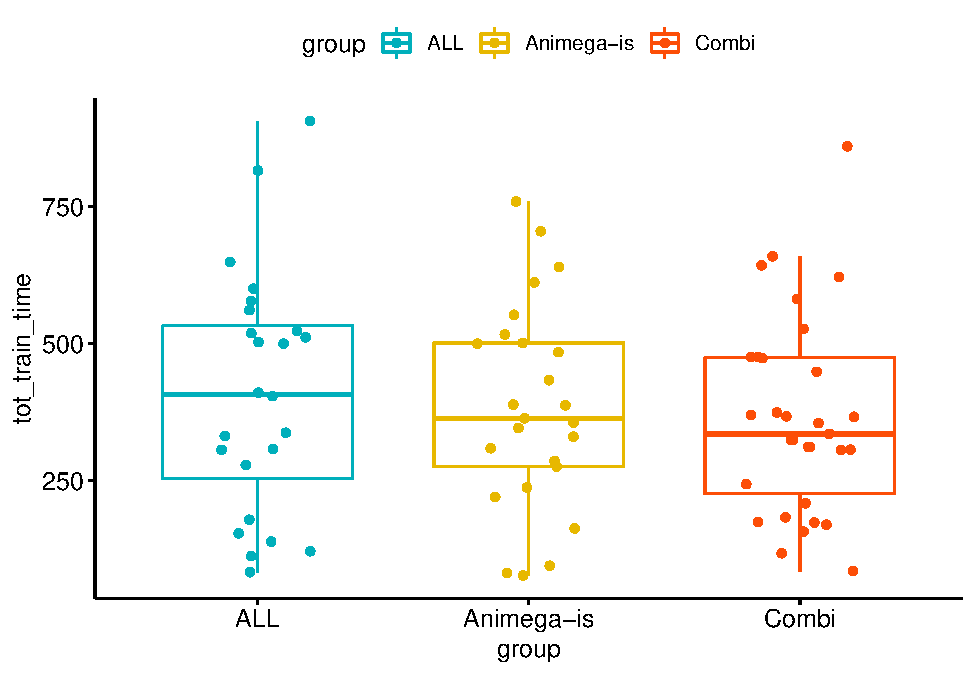
\includegraphics{Effects_of_training_files/figure-latex/tottraintime-plot-1.pdf}

\hypertarget{phonological-awareness-1}{%
\subsection{Phonological awareness}\label{phonological-awareness-1}}

\hypertarget{hypothesis-1-a-phonics-based-reading-strategy-improves-phonological-awareness.}{%
\subsubsection{Hypothesis 1: A phonics-based reading strategy improves
phonological
awareness.}\label{hypothesis-1-a-phonics-based-reading-strategy-improves-phonological-awareness.}}

There was almost a significant interaction between days and the
intervention on phonics-based reading, the group training phonic-based
strategies improved more than the comparison group
(\(\hat{\beta} = 0.01\), 95\% CI \([0.00, 0.02]\), \(t(361.28) = 1.71\),
\(p = .089\)).

\hypertarget{hypothesis-2-a-comprehension-based-reading-strategy-improves-phonological-awareness.}{%
\subsubsection{Hypothesis 2: A comprehension-based reading strategy
improves phonological
awareness.}\label{hypothesis-2-a-comprehension-based-reading-strategy-improves-phonological-awareness.}}

There was no significant interaction between days and intervention for
the comprehension-based reading strategy on PA (\(\hat{\beta} = 0.00\),
95\% CI \([0.00, 0.01]\), \(t(361.88) = 1.16\), \(p = .245\)).

\hypertarget{hypothesis-3-the-combination-of-both-reading-strategies-is-more-effective-than-either-strategy-on-its-own.}{%
\subsubsection{Hypothesis 3: The combination of both reading strategies
is more effective than either strategy on its
own.}\label{hypothesis-3-the-combination-of-both-reading-strategies-is-more-effective-than-either-strategy-on-its-own.}}

There was a significant interaction between the combined group and the
other two intervention groups, (\(\hat{\beta} = 0.01\), 95\% CI
\([0.00, 0.02]\), \(t(359.20) = 2.80\), \(p = .005\)), the combined
training improved PA over time more than the other two intervention
groups. The results from the PA models can be seen in
Table~@ref(tab:PA-table).

~

Effects of Interventions on Phonological Awareness

Predictors

Estimates

CI

p

(Intercept)

12.35

11.05~--~13.65

\textless0.001

Days

0.01

0.01~--~0.02

\textless0.001

Control vs PB

1.67

-0.47~--~3.81

0.125

Control vs CB

-0.42

-2.54~--~1.71

0.701

PB and CB vs Combi

0.80

-1.42~--~3.03

0.479

Days*Control vs PB

0.01

-0.00~--~0.02

0.089

Days*Control vs CB

0.00

-0.00~--~0.01

0.245

Days*PB and CB vs Combi

0.01

0.00~--~0.02

0.005

Random Effects

σ2

12.40

τ00 id

48.12

ICC

0.80

N id

132

Observations

489

Marginal R2 / Conditional R2

0.055 / 0.806

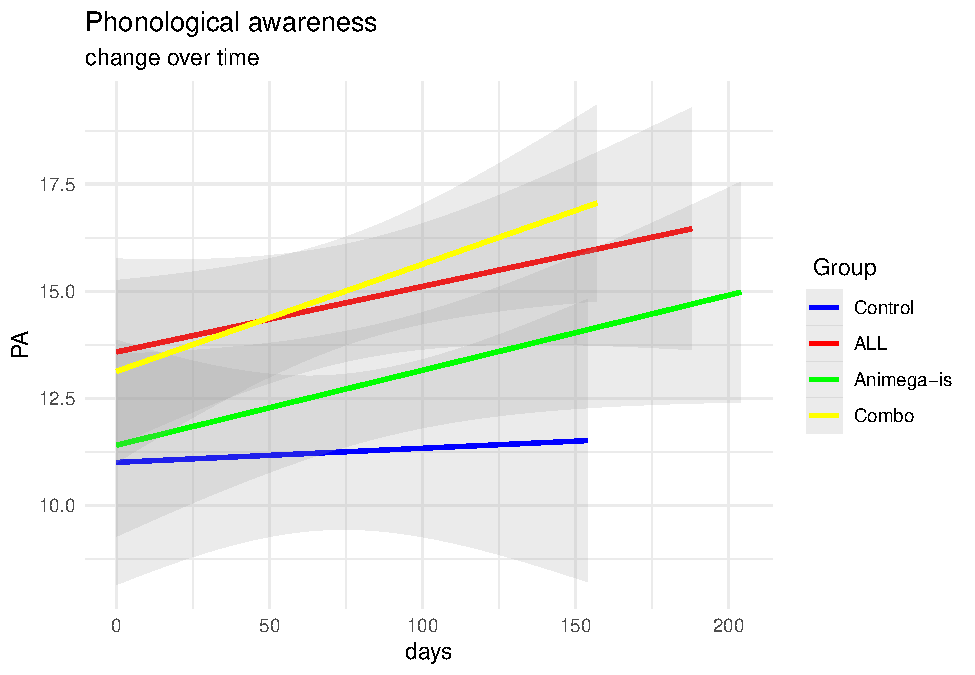
\includegraphics{Effects_of_training_files/figure-latex/PA-plot-1.pdf}

\hypertarget{word-recognition-1}{%
\subsection{Word recognition}\label{word-recognition-1}}

\hypertarget{hypothesis-1-a-phonics-based-reading-strategy-improves-word-recognition.}{%
\subsubsection{Hypothesis 1: A phonics-based reading strategy improves
word
recognition.}\label{hypothesis-1-a-phonics-based-reading-strategy-improves-word-recognition.}}

There was not a significant interaction between days and the
intervention on phonic-based-based reading (\(\hat{\beta} = 0.05\), 95\%
CI \([-0.05, 0.16]\), \(t(130.15) = 0.97\), \(p = .334\)).

\hypertarget{hypothesis-2-a-comprehension-based-reading-strategy-improves-word-recognition.}{%
\subsubsection{Hypothesis 2: A comprehension-based reading strategy
improves word
recognition.}\label{hypothesis-2-a-comprehension-based-reading-strategy-improves-word-recognition.}}

There was no significant interaction between days and intervention for
the comprehension-based reading strategy on word recognition
(\(\hat{\beta} = 0.00\), 95\% CI \([-0.10, 0.11]\),
\(t(117.30) = 0.06\), \(p = .955\)).

\hypertarget{hypothesis-3-the-combination-of-both-reading-strategies-is-more-effective-than-either-strategy-on-its-own.-1}{%
\subsubsection{Hypothesis 3: The combination of both reading strategies
is more effective than either strategy on its
own.}\label{hypothesis-3-the-combination-of-both-reading-strategies-is-more-effective-than-either-strategy-on-its-own.-1}}

There was a not significant interaction between the combined group and
the other two intervention groups, (\(\hat{\beta} = -0.01\), 95\% CI
\([-0.12, 0.10]\), \(t(164.42) = -0.17\), \(p = .867\)). The results
from the word models can be seen in Table~@ref(tab:word-table).

~

Effects of Interventions on Word Recognition

Predictors

Estimates

CI

p

(Intercept)

-0.18

-0.32~--~-0.04

0.012

Days

0.20

0.14~--~0.27

\textless0.001

Control vs PB

-0.01

-0.24~--~0.22

0.948

Control vs CB

0.15

-0.08~--~0.37

0.207

PB and CB vs Combi

0.15

-0.08~--~0.39

0.202

Days*Control vs PB

0.05

-0.05~--~0.16

0.333

Days*Control vs CB

0.00

-0.10~--~0.11

0.954

Days*PB and CB vs Combi

-0.01

-0.12~--~0.10

0.867

Random Effects

σ2

0.15

τ00 id

0.54

τ11 id.scale(days, center = FALSE)

0.02

ρ01 id

0.47

ICC

0.81

N id

131

Observations

485

Marginal R2 / Conditional R2

0.040 / 0.817

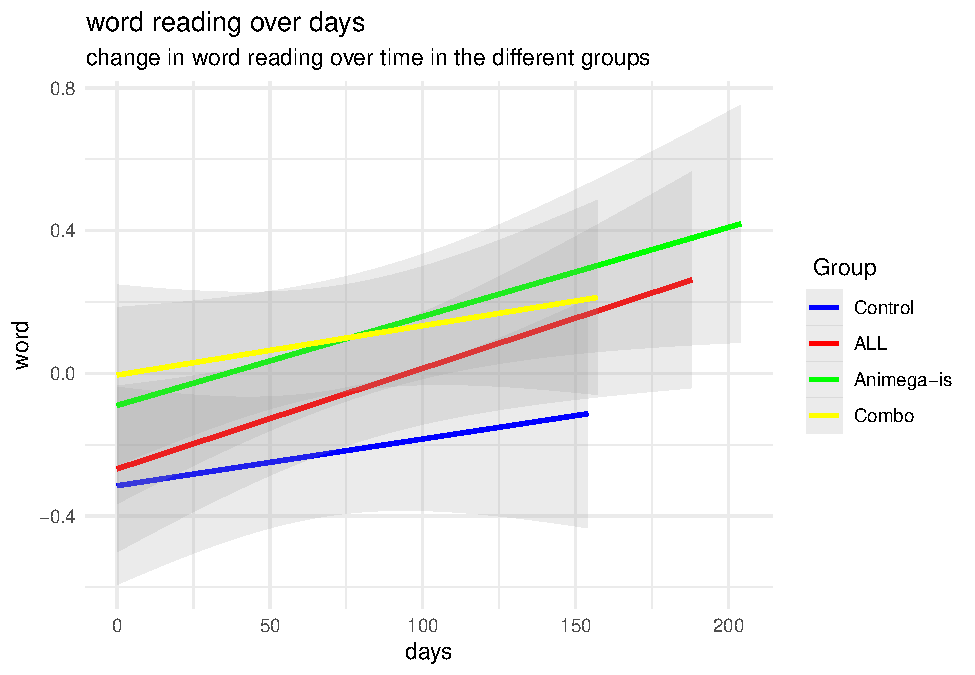
\includegraphics{Effects_of_training_files/figure-latex/word-plot-1.pdf}

\hypertarget{reading-comprehension-1}{%
\section{Reading comprehension}\label{reading-comprehension-1}}

\hypertarget{hypothesis-1-a-phonics-based-reading-strategy-improves-word-recognition.-1}{%
\subsubsection{Hypothesis 1: A phonics-based reading strategy improves
word
recognition.}\label{hypothesis-1-a-phonics-based-reading-strategy-improves-word-recognition.-1}}

There was not a significant interaction between days and the
intervention on phonic-based training on reading comprehension
(\(\hat{\beta} = 0.19\), 95\% CI \([-0.24, 0.62]\), \(z = 0.87\),
\(p = .383\)).

\hypertarget{hypothesis-2-a-comprehension-based-reading-strategy-improves-reading-comprehension.}{%
\subsubsection{Hypothesis 2: A comprehension-based reading strategy
improves reading
comprehension.}\label{hypothesis-2-a-comprehension-based-reading-strategy-improves-reading-comprehension.}}

There was no significant interaction between days and intervention for
the comprehension-based reading strategy on reading comprehension
(\(\hat{\beta} = -0.09\), 95\% CI \([-0.51, 0.33]\), \(z = -0.43\),
\(p = .668\)).

\hypertarget{hypothesis-3-the-combination-of-both-reading-strategies-is-more-effective-than-either-strategy-on-its-own.-2}{%
\subsubsection{Hypothesis 3: The combination of both reading strategies
is more effective than either strategy on its
own.}\label{hypothesis-3-the-combination-of-both-reading-strategies-is-more-effective-than-either-strategy-on-its-own.-2}}

There was a not significant interaction between the combined group and
the other two intervention groups, (\(\hat{\beta} = -0.13\), 95\% CI
\([-0.64, 0.38]\), \(z = -0.50\), \(p = .619\)).

The results from the word models can be seen in
Table~@ref(tab:DLS-table).

~

Effects of Interventions on Reading comprehension

Predictors

Incidence Rate Ratios

CI

p

(Intercept)

0.07

0.03~--~0.14

\textless0.001

Days

1.71

1.26~--~2.32

0.001

Control vs PB

1.07

0.45~--~2.54

0.885

Control vs CB

1.38

0.58~--~3.24

0.465

PB and CB vs Combi

0.89

0.36~--~2.24

0.812

Days*Control vs PB

1.21

0.79~--~1.86

0.383

Days*Control vs CB

0.91

0.60~--~1.39

0.668

Days*PB and CB vs Combi

0.88

0.53~--~1.46

0.619

Random Effects

σ2

2.38

τ00 id

5.38

τ11 id.scale(days, center = FALSE)

0.40

ρ01

~

ρ01

~

ICC

0.69

N id

131

Observations

484

Marginal R2 / Conditional R2

0.032 / 0.703

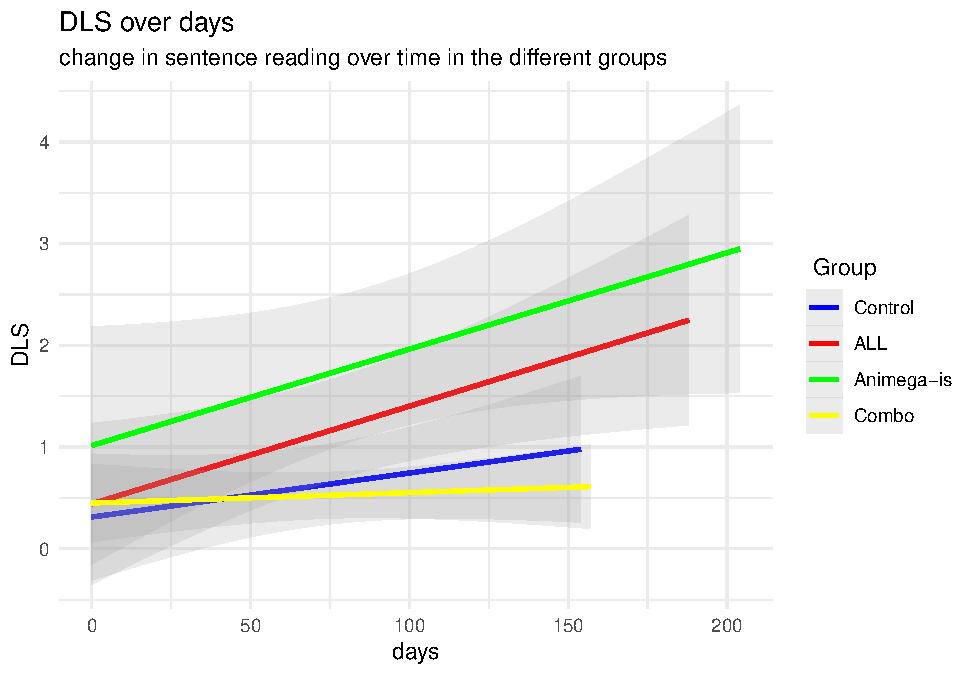
\includegraphics{Effects_of_training_files/figure-latex/DLS-plot-1.pdf}

\hypertarget{results-summary}{%
\section{Results summary}\label{results-summary}}

Both a phonic-based reading strategy and the combination of phonic-based
and comprehension-based reading strategies improves development in
phonological awareness more than teaching as usual. In addition, the
combination group had a steeper development in phonological awareness
than either reading strategy on its own. IQ influenced the starting
level of phonological awareness, word recognition, and reading
comprehension, and was marginally associated with the level of
improvement in phonological awareness. IQ and PA are important for
improving reading ability. IQ might be difficult to change but PA is
very much so. Thus, teachers in special needs school should include
phonic-based reading strategy training early and throughout school to
enable reading acquisition. phonic-based mer renodlad färdighetsträning
(alphabetic coding/phonological coding), som bidrar till ökad fonologisk
medvetenhet , comprehension-based bidrar till rikare lexico-semantic
representations. Kombinationen bidrar till att eleven får möjlighet att
tillämpa sina tillägnade färdigheter i en rik semantisk kontext.
Comprehension-based fokuserar för lite på färdigheten? Utebliven effekt
på word recognition talar kanske emot detta, men vi tror att det har att
göra med mängden träning och kanske nivån de startar på. Det beror inte
på mängden träning i studien (inga skillnader mellan grupperna) och inte
heller IQ (kontroll för det). ID-nivå? Ålder? Kön? Vad har andra sagt?
Om kombinerad träning och teoretiskt vad det representerar? Och
specifikt om comprehension-based?

\hypertarget{marginal-and-conditional-r2}{%
\section{marginal and conditional
R2}\label{marginal-and-conditional-r2}}

A marginal R2 close to zero tells us that the fixed effects aren't
explaining much variation, and a conditional R2 close to 1 tells us that
most of that unexplained variation is between groups (people) rather
than between observations within groups (people). So, for example, if
the context was a longitudinal cohort study, we wouldn't expect to
improve our model much by collecting more data on
characteristics/measures that mainly vary within people, but instead
should find characteristics that mainly vary between people.

\hypertarget{discussion}{%
\section{Discussion}\label{discussion}}

In the present study, we investigated whether reading interventions
targeting either phonic or comprehension-based reading strategies, or a
combination of both these strategies, improve reading skills in children
with ID, who use ACC. Our pre-registered hypothesis that either reading
strategy would improve phonological awareness (Hypothesis 1) was
supported by the results, and for the test on phonological awareness, we
also found support for Hypothesis 3, that the combined intervention
would reveal the steepest development. However, we did not see that
intervention improved word or reading comprehension skill (Hypothesis
2). Our exploratory analyses indicated \ldots{} . Reading intervention
might support reading skill development in children with ID who use ACC,
but the stages in development cannot be circumvented.

In line with earlier research, we found that reading can be taught to
students with ID. Our research adds a large-scale study including
students who also benefit from AAC, in practice children with lower
cognitive level (i.e.~IQ). Earlier literacy intervention studies for
students with ID have mainly included children with mild ID, and the
ones that have included moderate to severe have mostly been case
studies. Our study conclude that even though IQ is important for the
acquisition of reading, children with mild to moderate can also benefit
from literacy instruction.

Reading builds on several simultaneous processes, and training programs
on these instructional strategies inevitably overlap in the mechanisms
that they activate. For example, a comprehension-based instructional
strategy does not exclude the possibility to apply phonic-based
principles as the meaning of words are sought and when working with a
phonic-based approach, lexico-semantic processes (e.g., phonological
structures in the lexicon, semantic associations) might influence
training outcomes. Still, the emphasis is different across strategies,
and it is reasonable to assume that they support development in
different reading components.

\#\#Conclusions Blablabla

\#\#Declaration of interest Blablabla

\newpage

\hypertarget{references}{%
\section{References}\label{references}}

\begingroup
\setlength{\parindent}{-0.5in}
\setlength{\leftskip}{0.5in}

\hypertarget{refs}{}
\begin{CSLReferences}{0}{0}
\end{CSLReferences}

\endgroup

\end{document}
